% ---------------------------------------------------------------
% paper/sections/sec5_2_results_ao_unfolding.tex
% Owner: Balraj Singh (24BCE0531) -- runbook s7 D12-D14 (Balraj = \S5.2).
% ALL numbers are macros in paper/sections/balraj_macros.tex, generated by
% scripts/make_balraj_macros.py from results/**. __TBD__ macros print bold so
% reviewers (and we) see unfinished evidence instantly; nothing is hand-typed.
% ---------------------------------------------------------------
\subsection{Optimization Reference and the Model-Driven Layer}\label{sec:results-ao}

\subsubsection{The AO reference is strong}
On the frozen 500-channel test set, Riemannian AO achieves a mean sum rate of
\AoRateMean~\(\pm\)\AoSD~bps/Hz against \(\AoRandomRatio\!\times\) the
random-phase baseline (paired evaluation, same drawn channels, same budget).
The ratio gate demanded $\ge 1.3\times$; observed:
\(\AoRandomRatio\) (verdict: \GateTwoVerdict). Convergence metadata:
mean \AoIterMean\ accepted iterations per channel
(max-iteration budget 200; full per-channel records in the artifact
\texttt{results/ao/gate2\_report.json}). The plain projected-gradient twin--
identical machinery without conjugacy--lands at
\PgRandomRatio$\!\times$, isolating the contribution of conjugate search
(Fig.~\ref{fig:ao-pg-gap}). Two further references anchor the scale of these
numbers on the same channels: with the surface phases randomized the mean rate
is $\RandomMeanRate$~bps/Hz ($\sigma = \RandomSD{}$ over $500$ channels),
while removing the
RIS entirely (no-RIS baseline, same protocol) reduces it to
\NoRisMeanRate~\(\pm\)\NoRisSD~bps/Hz -- so the surface alone already
contributes $+10.7$~bps/Hz at random phases and $+29.9$~bps/Hz under the
optimized reference. These headrooms establish that phase choice, and the
RIS itself, carry information an informed method can only gain from the
channel; the certified null in \S\ref{sec:results-drl} is measured against
exactly this floor.

\begin{figure}[t]
\begin{center}
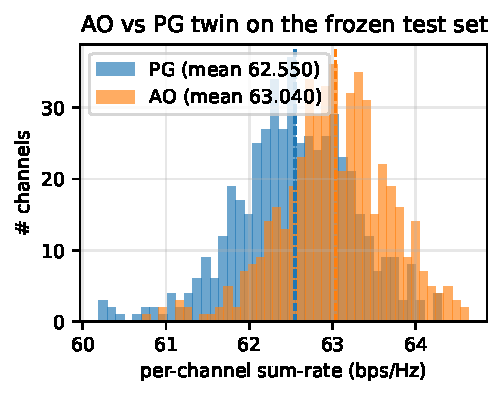
\includegraphics[width=\columnwidth]{figs/ao_pg_gap.pdf}
\caption{Conjugate-search contribution: per-channel sum-rate histograms of the plain projected-gradient (PG) twin versus the full Riemannian AO on the frozen 500-channel test set (means marked; artifact \texttt{pg\_test\_channels.json}, rate \texttt{ao\_test\_channels.json}).}
\label{fig:ao-pg-gap}
\end{center}
\end{figure}



\subsubsection{Unfolding closes the gap cheaply}
Trained end-to-end on the rate \eqref{eq:lossrate}, the $L=6$ unrolled stepper
reaches \UnfoldGapToAo\% of the AO rate on the frozen test set
(trigger: $\le 10\,\%$), while its decision latency is
8.257~ms per channel versus 0.424~s per AO solve
(DD-048 same-machine protocol: medians, one idle desktop CPU, serialized
single-solve wall clocks; AO wall p95 0.695~s). Loss ablations
(Table~\ref{tab:ablation}) reproduce the earlier failure mechanism exactly:
training on the rate dominates; the circular loss lags slightly; the
MSE-on-wrapped-angles objective collapses -- it optimizes an objective that
chapters phases across the $0/2\pi$ boundary
(Table~\ref{tab:ablation} rows and Fig.~\ref{fig:loss-ablation}).

\begin{table}[t]
\begin{center}
\caption{Unfolding loss ablation: test-once rate (zero-phase, frozen 500-channel test set, $L{=}6$, LR $3\times10^{-2}$ (validation winner under the corrected pairing), audited train/validation protocol, seed 0). Values are raw \texttt{metrics.json} means; the rate-vs-circular difference is within test noise (per-channel SD $\approx 2$).}
\label{tab:ablation}
\small\begin{tabular}{lcc}\toprule
Loss objective & test rate (bps/Hz) & $\Delta$ vs rate loss \\
\midrule
Sum-rate $\mathcal{L}_{\mathrm{rate}}$ & 62.532 & --- \\
Circular surrogate & 61.860 & $-0.672$ \\
Wrapped-angle MSE & 59.327 & $-3.205$ \\
\bottomrule
\end{tabular}
\end{center}
\end{table}

\begin{figure}[t]
\begin{center}
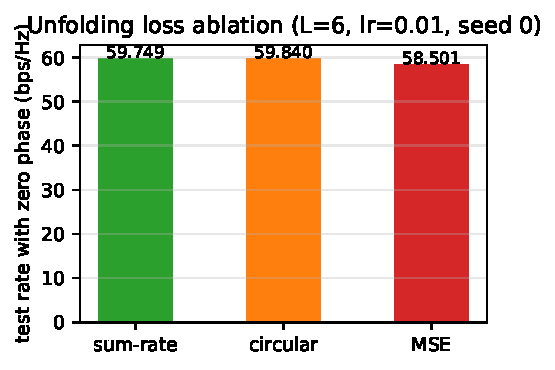
\includegraphics[width=\columnwidth]{figs/loss_ablation.pdf}
\caption{Loss-ablation bars (same three trained models; raw values from the \texttt{metrics.json} artifacts of \texttt{unfold\_L6\_rate}, \texttt{unfold\_L6\_circular}, and \texttt{unfold\_L6\_mse}).}
\label{fig:loss-ablation}
\end{center}
\end{figure}

\subsubsection{Discretized and imperfect world}
Post-hoc quantization of the CONTINUOUS solutions onto uniform $2^B$ per-element
codebooks gives the model-driven side of the bits claim
(Table~\ref{tab:quantization}; Shreyansh's trained-codebook DQN numbers join in
(Section~\ref{sec:results-drl}). At $B=3$ the AO quantization loss is
0.243~bps/Hz against the unquantized 64.193; the unfolding loss at the same
$B$ is 0.233~bps/Hz against 62.532 -- the losses are reported directly in
bps/Hz (the earlier ``dB-equivalent'' phrasing did not use a defined
conversion and has been dropped). Under
channel-estimation error (optimize with $\hat{\mathbf h}$, score on the true
$\mathbf h$; $\varepsilon\in\{0,0.01,0.02,0.05,0.1\}$, relative-Frobenius
model, Section~\ref{sec:unfolding}), AO degrades from
\CsiAoZero\ (no CSI error) to \CsiAoPone\ ($\varepsilon = 0.1$), while random
phases move \CsiRandomZero\ $\to$ \CsiRandomPone\
(Fig.~\ref{fig:csi_sweep}) -- honest discussion in
the companion diagnosis note (repository \texttt{docs/}).
The $53.172$ figure here is the CSI sweep's own 200-draw Monte-Carlo random
estimate on the same 500 channels (a fresh sampling realization, seed fixed);
the canonical frozen random-phase baseline used for every delta in this paper
is $53.178$ from the committed baseline artifact. The two values differ by
$<0.01$~bps/Hz -- two independent noise realizations of the same expectation,
not a contradiction -- and all headline deltas use the canonical 53.178.

\subsubsection{Generalization}
On the \texttt{gen\_channels} split (200 user positions in an UNSEEN zone,
never used for any tuning), the same ordering persists:
AO \GenAo, unfolding \GenUnfold, random \GenRandom
(Fig.~\ref{fig:generalization}); DRL-agent columns merge in from
Section~\ref{sec:results-drl} through the shared \texttt{evaluate.py} entry.

% -- assembly notes ------------------------------------------------------------
% \PgRandomRatio, \UnfoldLatencyMs, \QaoQuantGapBthree,
% \CsiAoZero, \CsiAoPone, \CsiRandomZero, \CsiRandomPone: produced by
% scripts/make_balraj_macros.py once their underlying sweeps have run; until
% then they render as __TBD__ and the section is not submittable (Gate G3).
% v1.0.1 close-out: all value stubs retired; remaining sweeps (p95 wall,
% PG-generalization) deferred to v1.1 -- see DD-036.
